\section{Active Directory Groups}
They can place similar users together and mass assign rights and access. Groups are another key target for attackers and penetration testers, as the rights that they confer on their members may not be readily apparent but may grant excessive (and even unintended) privileges that can be abused if not set up correctly. 

There are many built-in groups in Active Directoryo
The number of groups in an AD environment can snowball and become unwieldy, potentially leading to unintended access if left unchecked. 
It is essential to understand the impact of using different group types and for any organization to periodically audit which groups exist within their domain, the privileges that these groups grant their members, and check for excessive group membership beyond what is required for a user to perform their day-to-day work. 

Difference between Groups and Organizational Units (OUs): 
\begin{itemize}
        \item OU: OUs are useful for grouping users, groups, and computers:
            \begin{itemize}
                    \item to ease management and deploying Group Policy settings to specific objects in the domain. 
                    \item to delegate administrative tasks to a user, such as resetting passwords or unlocking user accounts without giving them additional admin rights that they may inherit through group membership.
            \end{itemize}
        \item Groups are primarily used to assign permissions to access resources
\end{itemize}

In simpler terms, groups are used to place users, computers, and contact objects into management units that provide ease of administration over permissions and facilitate the assignment of resources such as printers and file share access. For example, if an admin needs to assign 50 members of a department access to a new share drive, it would be time-consuming to add each user's account individually. Granting permissions this way would also make it more difficult to audit who has access to resources and difficult to clean up/revoke permissions. Instead, a sysadmin can either use an existing group or create a new group and grant that specific group permissions over the resource. From here, every user in the group will inherit the permissions based on their membership in the group. If the permissions need to be modified or revoked for one or more users, they could merely be removed from the group, leaving the other users unaffected and their permissions intact.

Groups in Active Directory have two fundamental characteristics: 
\begin{itemize}
        \item type: that defines the group's purpose;
        \item scope: shows how the group can be used within the domain or forest.
\end{itemize}


\subsection{Types of groups}
\subsubsection{Security groups}

type used to ease the assignment ofpermissions and rights to a collection of users instead. 

All users added to a security group will inherit any permissions assigned to
the group.

\subsubsection{Distribution groups}
The Distribution groups type is used by email applications to distribute messages to group members. 

This type of group cannot be used to assign permissions to resources in a domain environment.

\subsection{Scope of groups}
\begin{center}
\begin{figure}
    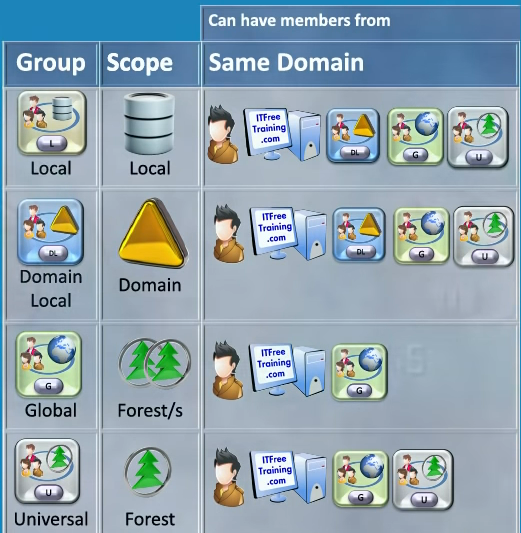
\includegraphics[width=0.5\linewidth]{windows_knowledge/ad/images/group-scopes.png}
  \caption{Group scopes overview}
  \label{fig:ad-group-scopes}
\end{figure}
\end{center}

Group scopes can be changed, but there are a few caveats:
\begin{itemize}
        \item A Global Group can only be converted to a Universal Group if it is NOT part of another Global Group.
        \item A Domain Local Group can only be converted to a Universal Group if the Domain Local Group does NOT contain any other Domain Local Groups as members.
        \item A Universal Group can be converted to a Domain Local Group without any restrictions.
        \item A Universal Group can only be converted to a Global Group if it does NOT contain any other Universal Groups as members.
\end{itemize}


\subsubsection{Domain Local}

\begin{itemize}
    \item Can only be used to manage permissions to domain resources in the domain where it was created.
    \item cannot be  used in other domains
    \item CAN contain users from OTHER domains
    \item can be nested into other local groups
    \item cannot be nested into global groups
\end{itemize}

\subsubsection{Global}
\begin{itemize}
    \item can be used to grant access to resources in another domain
    \item can only contain accounts from the domain where it was created.
    \item can be added to both other global groups and local groups
\end{itemize}

\subsubsection{Universal}
\begin{itemize}
    \item Can be used to manage resources distributed across multiple domains
    \item can be given permissions to any object within the same forest.
    \item are available to all domains within an organization
    \item can contain users from any domain.
    \item adding or removing objects from a universal group triggers forest-wide replication.
\end{itemize}

It is recommended that administrators maintain other groups (such as global groups) as members of universal groups because global group membership within universal groups is less likely to change than individual user membership in global groups.  Replication is only triggered at the individual domain level when a user is removed from a global group. 

\subsection{Built-in vs. Custom Groups}

Several
\href{https://docs.microsoft.com/en-us/windows/security/identity-protection/access-control/active-directory-security-groups}{built-in
security groups} are created with a Domain Local Group scope
when a domain is created.  These groups are used for specific administrative
purposes and are discussed more in the next section.  It is important to note
that only user accounts can be added to these built-in groups as they do not
allow for group nesting (groups within groups).

Some examples of built-in groups included Domain Admins, which is a Global security group and can only contain accounts from its own domain. 

If an organization wants to allow an account from domain B to perform administrative functions on a domain controller in domain A, the account would have to be added to the built-in Administrators group, which is a Domain Local group. 

Though Active Directory comes prepopulated with many groups, it is common for most organizations to create additional groups (both security and distribution) for their own purposes. Changes/additions to an AD environment can also trigger the creation of additional groups. For example, when Microsoft Exchange is added to a domain, it adds various different security groups to the domain, some of which are highly privileged and, if not managed properly, can be used to gain privileged access within the domain.
\subsection{Privileged Accounts and Groups}
This page has a detailed listing of
\href{https://docs.microsoft.com/en-us/windows-server/identity/ad-ds/plan/security-best-practices/appendix-b--privileged-accounts-and-groups-in-active-directory}{privileged accounts and groups} in Active Directory
\subsubsection{Backup Operators}
\subsubsection{Event Log Readers}
\subsubsection{DnsAdmins}
\subsubsection{Hyper-V Administrators}
\subsubsection{Print Operators}
\subsubsection{Server Operators}
\subsection{Nested Group Membership}

Nested group membership is an important concept in AD. As mentioned previously, a Domain Local Group can be a member of another Domain Local Group in the same domain. Through this membership, a user may inherit privileges not assigned directly to their account or even the group they are directly a member of, but rather the group that their group is a member of. This can sometimes lead to unintended privileges granted to a user that are difficult to uncover without an in-depth assessment of the domain. Tools such as BloodHound are particularly useful in uncovering privileges that a user may inherit through one or more nestings of groups. This is a key tool for penetration testers for uncovering nuanced misconfigurations and is also extremely powerful for sysadmins and the like to gain deep insights (visually) into the security posture of their domain(s).

\subsection{Scope Strategies}
\subsubsection{AGDLP}

ADDLP stands for:
\begin{itemize}
        \item A for Accounts.
        \item G for Global Group.
        \item DL for Domain Local Group.
        \item P for Permissions.
\end{itemize}

It is a role based strategy that is designed to provide flexible resource
management using groups. It is designed for larger networks (more than 500
users). AGDLP can be used in multiple domain environments but is generally used in a single domain environment.

Since AGDLP is a role base strategy for applying permissions, as a user changes their role in an organization, it is easy to change the permissions associated to that user by making them members of the appropriate groups. Since the users are being put into groups at the role level, this means that the administrator does not require knowledge of how the permissions were applied to the resource. Lastly, by looking at the users in the groups, you can quickly determine who has access to which resources in your domain.

The basic way to use AGDLP is as follows:
\begin{itemize}
    \item Accounts go into Global Groups; 
    \item Global Groups go into Domain Local Groups;
    \item Domain Local Groups are than applied to Permissions. 
\end{itemize}

The advantage to using each group is as follows:
\begin{itemize}
    \item Global Groups allow users from the same domain to be members. This means that when using multiple domains, you can be assured that only users and computers and other Global Groups from that domain are members. This means you can force administration to be divided up between domains. If you do not use Global Groups you could never be sure if an administrator from a domain is only adding users from that domain.
    \item Domain Local Groups can only be used in the domain that the group was created in. This helps with auditing. If the group could be used in other domains, you could never be sure that the group had been applied to resources outside your domain.
\end{itemize}

AGDLP can be used in a single forest, single domain environment and also a multi domain environment. 

\url{https://www.youtube.com/watch?v=zHHzjjqVhTc}

\subsubsection{AGUDLP}

What AGUDLP standards for
\begin{itemize}
        \item A Accounts
        \item G Global Groups
        \item U Universal Groups
        \item DL Domain Local Groups
        \item P Permissions
\end{itemize}


AGUDLP can be used in multiple domain environments to provide distributed control between different domain administrators while still being able to provide access to resources at the forest level.


It allows administration to be divided up between different administrators in the forest. Administrators can have control at the forest level or control can be  separated at  the domain or resources level.

Since AGUDLP is a role base strategy, when a user changes their role, for example promoted or transferred, access can quickly and easily  be changed.

AGUDLP also allows easy auditing. By looking in the group it can quickly be determined who has access to which resources.

Why each group is used:
\begin{itemize}
    \item Global groups only contain users, computers, and other global groups
        from the same domain. If we wanted a sales
            group that had all sales users from all domains in the forest, we
            would first create a global group for the sales users in each
            domain. This allows to divide up control between
        different domains and  domain administrators in each domain to be
        responsible for keeping this group up to date. 
    \item Universal groups allow users, computers, global groups and other
        universal groups to be members. Because of this, they can have the
        global groups from all the other domains to be members of this group.
        For example, a universal group could have as members  the sales group
        from all the other domains. Universal groups are available forest wide
        and thus are replicated using the global catalog server. For this
        reason, you will want to reduce replication as much as possible in the
        forest. Replication will only occur when membership of the universal
        group has changed. Since the universal group contains global groups,
        the membership of the global groups can change without affecting the
        membership of the universal group. The only time the universal group
        would need to be replicated is when a global group is added or removed
        from the universal group.

    \item The domain local group is applied to the resources as a permission.
    Domain local groups can only be used in the domain that they were created
    in. By using domain local groups, a local domain administrator can simply
    add the domain local group to the resources and configure the appropriate
    permissions. This administrator may not have access to change the
    membership of the other groups, which means that they do not have control
    over which users go into the group. This does not affect their ability to
    use the group on local resources. This means that by using a domain local
    group, the scope of the group can be limited to use for that domain only
    and also be delegated out to other administrators. At this level, it is
    easy to add or remove the universal group to any domain local group as
    required, making changing access very quick and flexible.
\end{itemize}

\url{https://www.youtube.com/watch?v=yjPGRnxAU6M}
